
\documentclass{article} 
% Pacchetti di Codifica e Lingua 
\usepackage[utf8]{inputenc} 
\usepackage[T1]{fontenc} 
\usepackage[italian]{babel} 
% Pacchetti Grafici e Diagrammi 
\usepackage{graphicx} 
\usepackage{tikz} 
\usepackage{tikz-3dplot} 
\usetikzlibrary{angles,quotes,arrows.meta, positioning} 
\usepackage{pgfplots} 
\pgfplotsset{compat=1.18} % Pacchetti Matematici 
\usepackage{amsmath, amssymb, amsthm} 
% Pacchetti per Tabelle e Unità di Misura 
\usepackage{geometry} 
\usepackage{siunitx} 
\usepackage{booktabs} 
\usepackage{tabularx} 
\usepackage{colortbl} 
\usepackage{adjustbox} 
% Pacchetti per Layout e Formattazione 
\usepackage{fancyhdr} 
\usepackage{float} 
\usepackage{microtype} 
% Altri Pacchetti Utili 
\usepackage{mdframed} 
\usepackage{animate} 
\usepackage{ulem} 
\usepackage{eurosym} 
% Pacchetto enumitem 
\usepackage{enumitem} 
% Definizioni dei Colori 
\definecolor{lightblue}{HTML}{9cd8fc} 
\definecolor{myblue}{HTML}{139FE9} 
\definecolor{myblack}{HTML}{303030} 
\definecolor{mygray}{HTML}{787878} 
\definecolor{mywhite}{HTML}{c7c7c7} 
%\pagecolor{myblack} 
%\color{mywhite} 
% Configurazioni di fancyhdr 
\pagestyle{fancy} 
\fancyhf{} 
% Pulisce tutti i campi 
\fancyhead[LO]{\nouppercase{\rightmark}} 
% Titolo della sezione 
\renewcommand{\headrulewidth}{0.5pt} 
\renewcommand{\footrulewidth}{0pt} 
\geometry{a4paper, left=20mm, right=20mm, top=20mm, bottom=20mm} 
% Pacchetto Hyperref (inserito per ultimo) 
\usepackage{hyperref}
% Additional Packages 
\usepackage{xparse,array}
\begin{document}
\section{Contabilità direzionale}
\begin{itemize}
    \item \textbf{Contabilità generale} : Processo di \textbf{rilevazione}, \textbf{misurazione}, \textbf{analisi}, \textbf{interpretazione} e \textbf{comunicazione} di informazioni che consentano agli utilizzatori (\textit{stakeholders}) di sviluppare \textbf{giudizi} e \textbf{decisioni} consapevoli riguardanti i loro rapporti con l’impresa.
    \item \textbf{Contabilità direzionale} : Processo che \textbf{produce informazioni},soprattutto quantitative, monetarie e non, utilizzate dal \textbf{management}, per favorire il raggiungimento degli obiettivi dell'organizzazione.\begin{itemize}
              \item \textbf{Programmazione} : definizione degli obiettivi e delle strategie per raggiungerli, attraverso la \textbf{pianificazione} delle attività, chiamato anche \textbf{budgeting}.
              \item \textbf{Implementazione} : attuazione delle decisioni prese.
              \item \textbf{Controllo} : verifica che le attività siano svolte in modo conforme alle decisioni prese.
          \end{itemize}
\end{itemize}
\subsection{Contabilità direzionale vs contabilità generale}
\begin{table}[H]
    \setlength{\extrarowheight}{12pt}
    \adjustbox{max width=\textwidth,center}{
        \centering
        \begin{tabular}{|l|l|l|}
            \hline
            \rowcolor{myblue}
            \textbf{Caratteristiche}       & \textbf{Contabilità direzionale}                       & \textbf{Contabilità generale}                             \\
            \hline
            \textbf{Necessità            } & Facoltativa                                            & Obbligatoria                                              \\
            \hline
            \textbf{Finalità             } & Strumento per assisitere il management nelle decisioni & Strumento per assisitere gli stakeholders nelle decisioni \\
            \hline
            \textbf{Utenti               } & Management (noti)                                      & Stakeholders (ignoti)                                     \\
            \hline
            \textbf{Struttura sottostante} & Cambia in base alle esigenze                           & Struttura fissa ($A = P + CN$)                            \\
            \hline
            \textbf{Fonte dei principi   } & Qualsiasi sia utile                                    & Codice civile e Principi contabili                        \\
            \hline
            \textbf{Prospettiva          } & Storica e prospettica                                  & Storica                                                   \\
            \hline
            \textbf{Tipo di informazioni } & Quantitative e qualitative, prevalentemente monetarie  & Quantitative, monetarie                                   \\
            \hline
            \textbf{Precisione           } & Bassa                                                  & Alta                                                      \\
            \hline
            \textbf{Periodicità          } & Qualsiasi sia utile                                    & Annuale                                                   \\
            \hline
            \textbf{Tempestività         } & Qualsiasi sia utile                                    & Entro 120 giorni dalla chiusura dell'esercizio            \\
            \hline
            \textbf{Oggetto              } & Impresa ma anche singoli prodotti, clienti, ecc.       & Impresa                                                   \\
            \hline
            \textbf{Responsabilità       } & Virtualmente nessuna                                   & Sempre presente                                           \\
            \hline
        \end{tabular}
    }
    \caption{Contabilità direzionale vs contabilità generale}
\end{table}
\subsection{I 3 scopi e i 3 modi di considerare i costi}
\begin{itemize}
    \item \textbf{Misurazione} $\Rightarrow$ \textbf{Costo pieno} : \textbf{costo} di un prodotto o servizio, \textbf{somma} di tutti i costi sostenuti per produrlo o fornirlo.
    \item \textbf{Controllo} $\Rightarrow$ \textbf{Costo per centro di responsabilità} : \textbf{costo} di un centro di responsabilità, \textbf{somma} di tutti i costi sostenuti per gestirlo.
    \item \textbf{Decisione} $\Rightarrow$ \textbf{Costo differenziale} : \textbf{costo} di una decisione, \textbf{differenza} tra i costi alternativi.
\end{itemize}
\newpage
\section{Classificazione dei costi in funzione del loro comportamento}
\subsection{Costi}
\subsubsection*{Classificazione costi}
\begin{itemize}
    \item \textbf{Costi variabili totali} (CVT): costi che variano in proporzione al volume di produzione.
    \item \textbf{Costi fissi totali} (CFT): costi che non variano in proporzione al volume di produzione, si dividono in:
          \begin{itemize}
              \item \textbf{Costi impegnati (costi da capacità)}: costi  dotano l’azienda di una certa \textbf{“capacità produttiva”}, la quale perdura fino alla dismissione della relativa risorsa impegnata, sono irreversibili.
              \item \textbf{Costi discrezionali}: costi che l’azienda può decidere di sostenere o meno durante la fase di \textbf{"budgeting"} sono reversibili.
          \end{itemize}
    \item \textbf{Costi semivariabili} : costi che sono un mix di costi fissi e costi variabili.
    \item \textbf{Costi viscosi} : costi che variano in modo discontinuo, crescono rapidamente in risposta a un aumento del volume di produzione, ma diminuiscono lentamente in risposta a una diminuzione del volume di produzione.
    \item \textbf{Costi a gradino} : costi riferiti a risorse che possono essere acquistate o vendute solo in quantità discrete.
\end{itemize}
\begin{figure}[H]
    \centering
    \begin{tikzpicture}[scale = 0.,
            declare function={
                    f(\x) = 1.5*\x + 1;
                    g(\x) = 1.5*\x;
                    h(\x) = + 1;
                }]
        \begin{axis}
            [
                xlabel={\( volume \)},
                ylabel={\( costo \)},
                xmin=0, xmax=5,
                ymin=0, ymax=5,
                grid=both,
                axis lines=middle,
                axis line style=->,
                grid style={line width=.1pt, draw=gray!10},
                major grid style={line width=.2pt,draw=gray!50},
                minor tick num=3,
                enlargelimits={abs=0.5},
                xlabel style={at={(ticklabel* cs:1)}, anchor=north west},
                ylabel style={at={(ticklabel* cs:1)}, anchor=south west},
                samples=100,
                unbounded coords=jump,
                legend pos=south east
            ]
            \addplot[domain=0:5, ultra thick, smooth, color=red]{g(x)};
            \addplot[domain=0:5, ultra thick, smooth, color=orange]{h(x)};
            \addplot[domain=0:5, ultra thick, smooth, color=myblue]{f(x)};
            \legend{$Costo\ variabile$, $Costo\ fisso$, $Costo\ semivariabile$}
        \end{axis}
    \end{tikzpicture}
    \begin{tikzpicture}[scale = 0.5,
            declare function={
                    f(\x) = \x;
                    g(\x) = 2*\x-2;
                }]
        \begin{axis}
            [
                xlabel={\( volume \)},
                ylabel={\( costo \)},
                xmin=0, xmax=5,
                ymin=0, ymax=5,
                grid=both,
                axis lines=middle,
                axis line style=->,
                grid style={line width=.1pt, draw=gray!10},
                major grid style={line width=.2pt,draw=gray!50},
                minor tick num=3,
                enlargelimits={abs=0.5},
                xlabel style={at={(ticklabel* cs:1)}, anchor=north west},
                ylabel style={at={(ticklabel* cs:1)}, anchor=south west},
                samples=100,
                unbounded coords=jump,
                legend pos=south east
            ]
            \addplot[domain=0:2, ultra thick, smooth, color=red]{f(x)};
            \addplot[domain=2:5, ultra thick, smooth, color=red]{g(x)};
            \legend{$Costo\ viscoso$}
        \end{axis}
    \end{tikzpicture}
    \begin{tikzpicture}[scale = 0.5,
            declare function={
                    f(\x) = ceil(\x);
                    g(\x) = \x;
                }]
        \begin{axis}
            [
                xlabel={\( volume \)},
                ylabel={\( costo \)},
                xmin=0, xmax=5,
                ymin=0, ymax=5,
                grid=both,
                axis lines=middle,
                axis line style=->,
                grid style={line width=.1pt, draw=gray!10},
                major grid style={line width=.2pt,draw=gray!50},
                minor tick num=3,
                enlargelimits={abs=0.5},
                xlabel style={at={(ticklabel* cs:1)}, anchor=north west},
                ylabel style={at={(ticklabel* cs:1)}, anchor=south west},
                samples=100,
                unbounded coords=jump,
                legend pos=south east
            ]
            \addplot[domain=0:5, ultra thick, smooth, color=myblue]{f(x)};
            \addplot[domain=0:5, dashed, thick, smooth, color=myblue!60]{g(x)};
            \legend{$Costo\ a\ gradino$, $Approssimazione\ lineare$}
        \end{axis}
    \end{tikzpicture}
    \caption{Classificazione costi}
\end{figure}

\begin{table}[H]
    \setlength{\extrarowheight}{10pt}
    \adjustbox{max width=\textwidth,center}{
        \centering
        \begin{tabular}{|l|l|l|l|}
            \hline
            \rowcolor{myblue}
            \textbf{Costo}           & \textbf{Equazione}                & \textbf{Spiegazione}                                    & \textbf{Osservazioni}                                                                 \\
            \hline
            Volume                   & $X$                               & Volume di produzione                                    & $\textcolor{myblue}{x}$                                                               \\
            \hline
            Costo variabile unitario & $cvu$                             & Costo per unità prodotta                                & $\textcolor{myblue}{m}$                                                               \\
            \hline
            Costo variabile totale   & $CVT = cvu \cdot X$               & Costi \textbf{complessivamente} proporzionali al volume & $CVT(\textcolor{myblue}{x}) = cvu \cdot \textcolor{myblue}{x}$                        \\
            \hline
            Costo fisso totale       & $CFT$                             & Costi \textbf{non} proporzionali al volume              & $CFT = \textcolor{myblue}{q}$                                                         \\
            \hline
            Costo totale             & $CT = CFT + cvu \cdot X$          & Somma dei costi \textbf{fissi} e \textbf{variabili}     & $CT(\textcolor{myblue}{x}) = CFT + cvu \cdot \textcolor{myblue}{x}$                   \\
            \hline
            Costo medio unitario     & $CMU = \displaystyle\frac{CT}{X}$ & Costo medio per unità prodotta                          & $\displaystyle CMU(\textcolor{myblue}{x}) = \frac{CFT} {\textcolor{myblue}{x}} + cvu$ \\
            \hline
        \end{tabular}
    }
    \caption{Costi}
\end{table}
\begin{figure}[H]
    \centering
    \begin{tikzpicture}[scale = 0.8,
            declare function={
                    f(\x) = 1.5*\x + 1;
                    g(\x) = 1.5*\x;
                    h(\x) = + 1;
                }]
        \begin{axis}
            [
                xlabel={\( volume \)},
                ylabel={\( costo \)},
                xmin=0, xmax=5,
                ymin=0, ymax=5,
                grid=both,
                axis lines=middle,
                axis line style=->,
                grid style={line width=.1pt, draw=gray!10},
                major grid style={line width=.2pt,draw=gray!50},
                minor tick num=3,
                enlargelimits={abs=0.5},
                xlabel style={at={(ticklabel* cs:1)}, anchor=north west},
                ylabel style={at={(ticklabel* cs:1)}, anchor=south west},
                samples=100,
                unbounded coords=jump,
                legend pos=south east
            ]
            \addplot[domain=0:5, dashed, thick, smooth, color=red]{g(x)};
            \addplot[domain=0:5, dashed, thick, smooth, color=orange]{h(x)};
            \addplot[domain=0:5, ultra thick, smooth, color=myblue]{f(x)};
            \legend{$CVT$, $CFT$, $CT$}
        \end{axis}
    \end{tikzpicture}
    \caption{Costo totale}
\end{figure}
\subsection{Costo medio unitario}
Il costo medio unitario è il costo medio per unità prodotta,
\begin{align*}
     & CMU                         = \frac{CT}{X} = \frac{CFT}{X} + cvu                                                                                                                                                                                    \\                                                                                                                          \\
     & CMU(\textcolor{myblue}{x})  =\frac{CT}{\textcolor{myblue}{x}} = \frac{CFT + CVT }{\textcolor{myblue}{x}}=\frac{CFT}{\textcolor{myblue}{x}} + \frac{cvu \cdot \textcolor{myblue}{x}}{\textcolor{myblue}{x}} =\frac{CFT}{\textcolor{myblue}{x}} + cvu \\
\end{align*}
\begin{figure}[H]
    \centering
    \begin{tikzpicture}[scale = 0.6,
            declare function={
                    f(\x) = 1.5 +1/\x ;
                    g(\x) = 1.5;
                }]
        \begin{axis}
            [
                xlabel={\( volume \)},
                ylabel={\( costo \)},
                xmin=0, xmax=5,
                ymin=0, ymax=5,
                grid=both,
                axis lines=middle,
                axis line style=->,
                grid style={line width=.1pt, draw=gray!10},
                major grid style={line width=.2pt,draw=gray!50},
                minor tick num=3,
                enlargelimits={abs=0.5},
                xlabel style={at={(ticklabel* cs:1)}, anchor=north west},
                ylabel style={at={(ticklabel* cs:1)}, anchor=south west},
                samples=100,
                unbounded coords=jump,
                legend pos=south east
            ]
            \addplot[domain=0.1:5, dashed, thick, smooth, color=red]{g(x)};
            \addplot[domain=0.1:5, ultra thick, smooth, color=myblue]{f(x)};
            \legend{$cvu$, $CMU$}
        \end{axis}
    \end{tikzpicture}
    \caption{Costo medio unitario}
\end{figure}
\subsection{Margine di contribuzione}
\subsubsection*{Ricavo unitario o Prezzo di vendita}
\begin{align*}
     & p \quad \text{o} \quad r_u
\end{align*}
È il ricavo ottenuto dalla vendita di una singola unità di prodotto.
\subsubsection*{Ricavo totale}
\begin{align*}
     & RT =  p \cdot X                                              \\
     & RT(\textcolor{myblue}{x}) =  p \cdot (\textcolor{myblue}{x})
\end{align*}
Indica il ricavo complessivo ottenuto dalla vendita di $X$ unità di prodotto.
\subsubsection*{Margine di contribuzione unitario}
\begin{align*}
     & MdC_u = (p - cvu) \\
\end{align*}
È la differenza tra il prezzo di vendita unitario e il costo variabile unitario.
\subsubsection*{Margine di contribuzione totale}
\begin{align*}
     & MdC_u =  RT - CVT =  (p - cvu) \cdot X                                                                                          \\
     & MdC(\textcolor{myblue}{x}) =  RT(\textcolor{myblue}{x}) - CVT(\textcolor{myblue}{x}) =  (p - cvu) \cdot (\textcolor{myblue}{x})
\end{align*}
Rappresenta il contributo totale alla copertura dei costi fissi e al profitto.
\subsubsection*{Margine di contribuzione percentuale}
\begin{align*}
     & \text{MCP} = \left( \frac{MdC_u}{p} \right) \cdot 100                            \\
     & \text{MCP}(\textcolor{myblue}{x}) = \left( \frac{(p - cvu)}{p} \right) \cdot 100
\end{align*}
Indica quale percentuale del prezzo di vendita per unità rimane dopo aver coperto i costi variabili unitari. È utile per determinare quanto ogni unità venduta contribuisca, in termini percentuali, alla copertura dei costi fissi e alla generazione di profitto.
\subsubsection*{Margine di sicurezza}
\begin{align*}
     & MS = X - X_P = X - \frac{CFT}{MdC_u} = \frac{MdC_u \cdot X - CFT}{MdC_u} = \frac{MdC - CFT}{MdC_u}                                                                             \\
     & MS(\textcolor{myblue}{x}) = \textcolor{myblue}{x} - \frac{CFT}{MdC_u} = \frac{MdC_u \cdot \textcolor{myblue}{x} - CFT}{MdC_u} = \frac{MdC(\textcolor{myblue}{x}) - CFT}{MdC_u}
\end{align*}
Rappresenta di quanto il volume attuale eccede il volume di pareggio.
\subsubsection*{Utile o Profitto}
\begin{align*}
     & P = RT - CT = MdC - CFT = (p - cvu) \cdot X  - CFT                                                        \\
     & P(\textcolor{myblue}{x}) = MdC(\textcolor{myblue}{x}) - CFT = (p - cvu) \cdot (\textcolor{myblue}{x})-CFT
\end{align*}
È la differenza tra il ricavo totale e il costo totale.
\subsubsection*{Volume di pareggio (Break-even volume)}
\begin{align*}
     & P(\textcolor{myblue}{x}) = 0                               \\
     & (p - cvu) \cdot (\textcolor{myblue}{x})-CFT = 0            \\
     & (p - cvu) \cdot (\textcolor{myblue}{x}) = CFT              \\
     & (\textcolor{myblue}{x}) = \displaystyle\frac{CFT}{(p-cvu)} \\
     & X_p = \displaystyle\frac{CFT}{MdC_u} = \frac{CFT}{(p-cvu)}
\end{align*}
Indica il volume di produzione necessario per coprire tutti i costi, generando un profitto nullo.
\subsubsection*{Volume per ottenere un profitto obiettivo}
\begin{align*}
     & P(\textcolor{myblue}{x}) = P_O                                             \\
     & (p - cvu) \cdot (\textcolor{myblue}{x})-CFT = P_O                          \\
     & (p - cvu) \cdot (\textcolor{myblue}{x}) = CFT + P_O                        \\
     & (\textcolor{myblue}{x}) = \displaystyle\frac{CFT + P_O}{(p-cvu)}           \\
     & X_{P_O} = \displaystyle\frac{CFT + P_O}{MdC_u} = \frac{CFT + P_O}{(p-cvu)}
\end{align*}
È il volume di produzione necessario per raggiungere un profitto obiettivo $P_O$.
\subsubsection*{Leva operativa}
L'effetto leva è misurato dal grado di leva operativa, che è il rapporto tra il margine di contribuzione e il profitto.
\begin{align*}
     & \text{Grado di leva operativa} = \frac{MdC}{P} = \frac{MdC_u \cdot X}{MdC_u \cdot X - CFT} = \frac{(p-cvu) X}{(p-cvu) X - CFT}                                                                                                                                                                                                                 \\
     & \text{Grado di leva operativa}(\textcolor{myblue}{x}) = \displaystyle\frac{MdC(\textcolor{myblue}{x})}{P(\textcolor{myblue}{x})} = \displaystyle\frac{MdC_u \cdot (\textcolor{myblue}{x})}{MdC_u \cdot (\textcolor{myblue}{x}) - CFT} = \displaystyle\frac{(p-cvu) \cdot (\textcolor{myblue}{x})}{(p-cvu) \cdot (\textcolor{myblue}{x}) - CFT} \\
\end{align*}
Indica di quanto varia il margine di contribuzione per unità di prodotto in risposta a una variazione del volume di produzione.
\subsection*{Incidenza percentuale delle quantità di vendita di un prodotto sulle quantità complessive}
\begin{align*}
     & I_{\% a} = \frac{X_a}{X_T} \cdot 100                                                \\
     & I_{\% (\textcolor{myblue}{x})} = \frac{(\textcolor{myblue}{x})}{\sum X_i} \cdot 100
\end{align*}
\subsubsection*{Margine di contribuzione equivalente}
\begin{align*}
     & MdC_e = \displaystyle MdC_a \cdot I_{\% a} + MdC_b \cdot I_{\% b} = (p_a - cvu_a) \cdot I_{\% a} + (p_b - cvu_b) \cdot I_{\% b} \\
\end{align*}
Se l'azienda ha più prodotti, il margine di contribuzione equivalente è la somma dei margini di contribuzione di tutti i prodotti, pesati per l'incidenza percentuale delle quantità di vendita di un prodotto sulle quantità complessive.
\subsubsection*{Tempo di produzione totale di produzione o Tempo macchina}
Indica il tempo di utilizzo di una macchina.
\subsubsection*{Tempo di produzione unitario}
\begin{align*}
     & T_u = \text{Tempo di produzione unitario} = \frac{\text{Tempo totale di produzione}}{\text{Numero di unità prodotte}} = \frac{\text{Tempo totale di produzione}}{(\textcolor{myblue}{x})} \\
     & T_u = \text{Tempo di produzione unitario} = \frac{1}{\text{Produttività oraria}} = \frac{1}{P_h}                                                                                          \\
\end{align*}
Indica il tempo necessario per produrre una singola unità di prodotto.
\subsubsection*{Produttività oraria}
\begin{align*}
     & P_h = \text{Produttività oraria} = \frac{\text{Numero di unità prodotte}}{\text{Tempo totale di produzione}} = \frac{(\textcolor{myblue}{x})}{\text{Tempo totale di produzione}} \\
     & P_h = \text{Produttività oraria} = \frac{1}{\text{Tempo di produzione unitario}} = \frac{1}{T_u}                                                                                 \\
\end{align*}
Indica il numero di unità prodotte in un'ora.
\subsubsection*{Margine di contribuzione orario}
\begin{align*}
     & MdC_h = \text{Margine di contribuzione orario} = \displaystyle\frac{MdC_{u}}{T_{u}} = MdC_u \cdot P_h \\
\end{align*}
Indica il margine di contribuzione per unità di tempo.
Lo uso quando negli esercizi mi viene dato un tempo macchina limite e devo capire quale mix di prodotti mi permette di massimizzare il margine di contribuzione.
\begin{table}[H]
    \setlength{\extrarowheight}{12pt}
    \adjustbox{max width=\textwidth,center}{
        \centering
        \begin{tabular}{|l|l|l|}
            \hline
            \rowcolor{myblue}
            \textbf{Voce}                                                       & \textbf{Spiegazione}                                                  & \textbf{Osservazioni}                                                                                                                                                                                                         \\
            \hline
            Ricavo unitario o Prezzo di vendita                                 & Ricavo per unità prodotta                                             & $\textcolor{myblue}{m}$                                                                                                                                                                                                       \\
            \hline
            Ricavo totale                                                       & Ricavi \textbf{complessivamente} proporzionali al volume              & $RT(\textcolor{myblue}{x}) = p \cdot \textcolor{myblue}{x}$                                                                                                                                                                   \\
            \hline
            Margine di contribuzione unitario                                   & Margine di contribuzione per unità prodotta                           & $MdC_u = (p - cvu)$                                                                                                                                                                                                           \\
            \hline
            Margine di contribuzione                                            & Ricavo totale - Costo variabile totale                                & $MdC(\textcolor{myblue}{x}) = RT(\textcolor{myblue}{x}) - CVT(\textcolor{myblue}{x}) = (p-cvu)(\textcolor{myblue}{x})$                                                                                                        \\
            \hline
            Margine di contribuzione percentuale                                & Percentuale del ricavo netto dai costi variabili per unità            & $ MdC_{\%}(\textcolor{myblue}{x}) = \left( \displaystyle\frac{(p - cvu)}{p} \right) \cdot 100$                                                                                                                                \\
            \hline
            Utile o Profitto                                                    & Ricavo totale - Costo totale                                          & $P(\textcolor{myblue}{x}) = MdC(\textcolor{myblue}{x}) - CFT = (p - cvu)(\textcolor{myblue}{x})-CFT$                                                                                                                          \\
            \hline
            Volume di pareggio                                                  & Volume di produzione per cui il profitto è nullo                      & $ (\textcolor{myblue}{x}) = \displaystyle\frac{CFT}{(p-cvu)}$                                                                                                                                                                 \\
            \hline
            Voleme per ottenere un profitto obiettivo $\textcolor{myblue}{P_O}$ & Volume di produzione per cui il profitto è $\textcolor{myblue}{P_O}$  & $ (\textcolor{myblue}{x}) = \displaystyle\frac{CFT + \textcolor{myblue}{P_O}}{(p-cvu)}$                                                                                                                                       \\
            \hline
            Grado di leva operativa                                             & Rapporto tra margine di contribuzione e profitto                      & $\text{Grado di leva}(\textcolor{myblue}{x}) = \displaystyle\frac{MdC(\textcolor{myblue}{x})}{P(\textcolor{myblue}{x})} = \displaystyle\frac{MdC_u \cdot (\textcolor{myblue}{x})}{MdC_u \cdot (\textcolor{myblue}{x}) - CFT}$ \\
            \hline
            Incidenza                                                           & Percentuale di un prodotto sul totale                                 & $I_{\% (\textcolor{myblue}{x})} = \displaystyle\frac{(\textcolor{myblue}{x})}{\sum X_i}$                                                                                                                                      \\
            \hline
            Margine di contribuzione equivalente                                & Somma dei margini di contribuzione pesati per l'incidenza percentuale & $MdC_e = \displaystyle MdC_a \cdot \frac{X_a}{X_{tot}} + MdC_b \cdot \frac{X_b}{X_{tot}}$                                                                                                                                     \\
            \hline
            Tempo di produzione unitario                                        & Tempo necessario per produrre una singola unità di prodotto           & $T_u = \displaystyle\frac{\text{Tempo totale di produzione}}{(\textcolor{myblue}{x})} = \displaystyle \frac{1}{P_h}$                                                                                                          \\
            \hline
            Produttività oraria                                                 & Numero di unità prodotte in un'ora                                    & $P_h = \displaystyle\frac{(\textcolor{myblue}{x})}{\text{Tempo totale di produzione}} = \displaystyle \frac{1}{T_u} $                                                                                                         \\
            \hline
            Margine di contribuzione orario                                     & Margine di contribuzione per unità di tempo                           & $MdC_h = \displaystyle\frac{MdC_{u}}{T_{u}} = MdC_u \cdot P_h$                                                                                                                                                                \\
            \hline
        \end{tabular}
    }
    \caption{Tabella di analisi del margine di contribuzione}
\end{table}

\subsection{Diagrammi di costo,ricavo e profitto}
\begin{figure}[H]
    \centering
    \begin{tikzpicture}[scale = 1,
            declare function={
                    f(\x) = 0.8*\x + 1;
                    g(\x) = 1.5*\x;
                }]
        \def\p{1.428}
        \begin{axis}
            [
                xlabel={\( volume \)},
                ylabel={\( costo\ o\ ricavi\)},
                xmin=-3, xmax=5,
                ymin=-3, ymax=5,
                grid=both,
                axis lines=middle,
                axis line style=->,
                grid style={line width=.1pt, draw=gray!10},
                major grid style={line width=.2pt,draw=gray!50},
                minor tick num=3,
                enlargelimits={abs=0.5},
                xlabel style={at={(ticklabel* cs:1)}, anchor=north west},
                ylabel style={at={(ticklabel* cs:1)}, anchor=south west},
                samples=100,
                unbounded coords=jump,
                legend pos=south east
            ]
            \coordinate (A) at (axis cs:\p,{f(\p)});
            \coordinate (B) at (axis cs:5,{f(5)});
            \coordinate (C) at (axis cs:5,{g(5)});
            \coordinate (D) at (axis cs: 0,{f(0)});
            \coordinate (E) at (axis cs: 0,{g(0)});
            \fill[gray, opacity=0.5] (A) -- (B) -- (C) -- cycle;
            \fill[gray, opacity=0.5] (A) -- (D) -- (E) -- cycle;
            \addplot[domain=0:5, ultra thick, smooth, color=myblue]{g(x)};
            \addplot[domain=0:5, ultra thick, smooth, color=red]{f(x)};
            \draw [dashed, thick, color=gray] (axis cs: \p, {f(\p)}) -- (axis cs: \p, 0);
            \filldraw[color=myblue] (axis cs: \p, {f(\p)}) circle (1.5pt);
            \node[below] at (axis cs: \p, 0) {\(X_P\)};
            \legend{$RT(x) = p \cdot (x)$, $CT(x) = CFT + cvu \cdot (x)$}
        \end{axis}
    \end{tikzpicture}
    \begin{tikzpicture}[scale = 1,
            declare function={
                    f(\x) = (1.5-0.8)*\x - 1;
                    g(\x) = 0;
                }]
        \def\p{1.428}
        \begin{axis}
            [
                xlabel={\( volume \)},
                ylabel={\( reddito \)},
                xmin=-3, xmax=5,
                ymin=-3, ymax=5,
                grid=both,
                axis lines=middle,
                axis line style=->,
                grid style={line width=.1pt, draw=gray!10},
                major grid style={line width=.2pt,draw=gray!50},
                minor tick num=3,
                enlargelimits={abs=0.5},
                xlabel style={at={(ticklabel* cs:1)}, anchor=north west},
                ylabel style={at={(ticklabel* cs:1)}, anchor=south west},
                samples=100,
                unbounded coords=jump,
                legend pos=south east,
            ]
            \coordinate (A) at (axis cs:\p,{f(\p)});
            \coordinate (B) at (axis cs:5,{f(5)});
            \coordinate (C) at (axis cs:5,{g(5)});
            \coordinate (D) at (axis cs: 0,{f(0)});
            \coordinate (E) at (axis cs: 0,{g(0)});
            \fill[gray, opacity=0.5] (A) -- (B) -- (C) -- cycle;
            \fill[gray, opacity=0.5] (A) -- (D) -- (E) -- cycle;
            \addplot[domain=0:5, ultra thick, smooth, color=myblue]{f(x)};
            \addplot[domain=0:5, ultra thin, smooth, color=gray]{g(x)};
            \draw [dashed, thick, color=gray] (axis cs: \p, {f(\p)}) -- (axis cs: \p, 0);
            \filldraw[color=myblue] (axis cs: \p, {f(\p)}) circle (1.5pt);
            \node[below] at (axis cs: \p, 0) {\(X_P\)};
            \legend{$P(x) = (p - cvu) \cdot (x) - CFT$}
        \end{axis}
    \end{tikzpicture}
    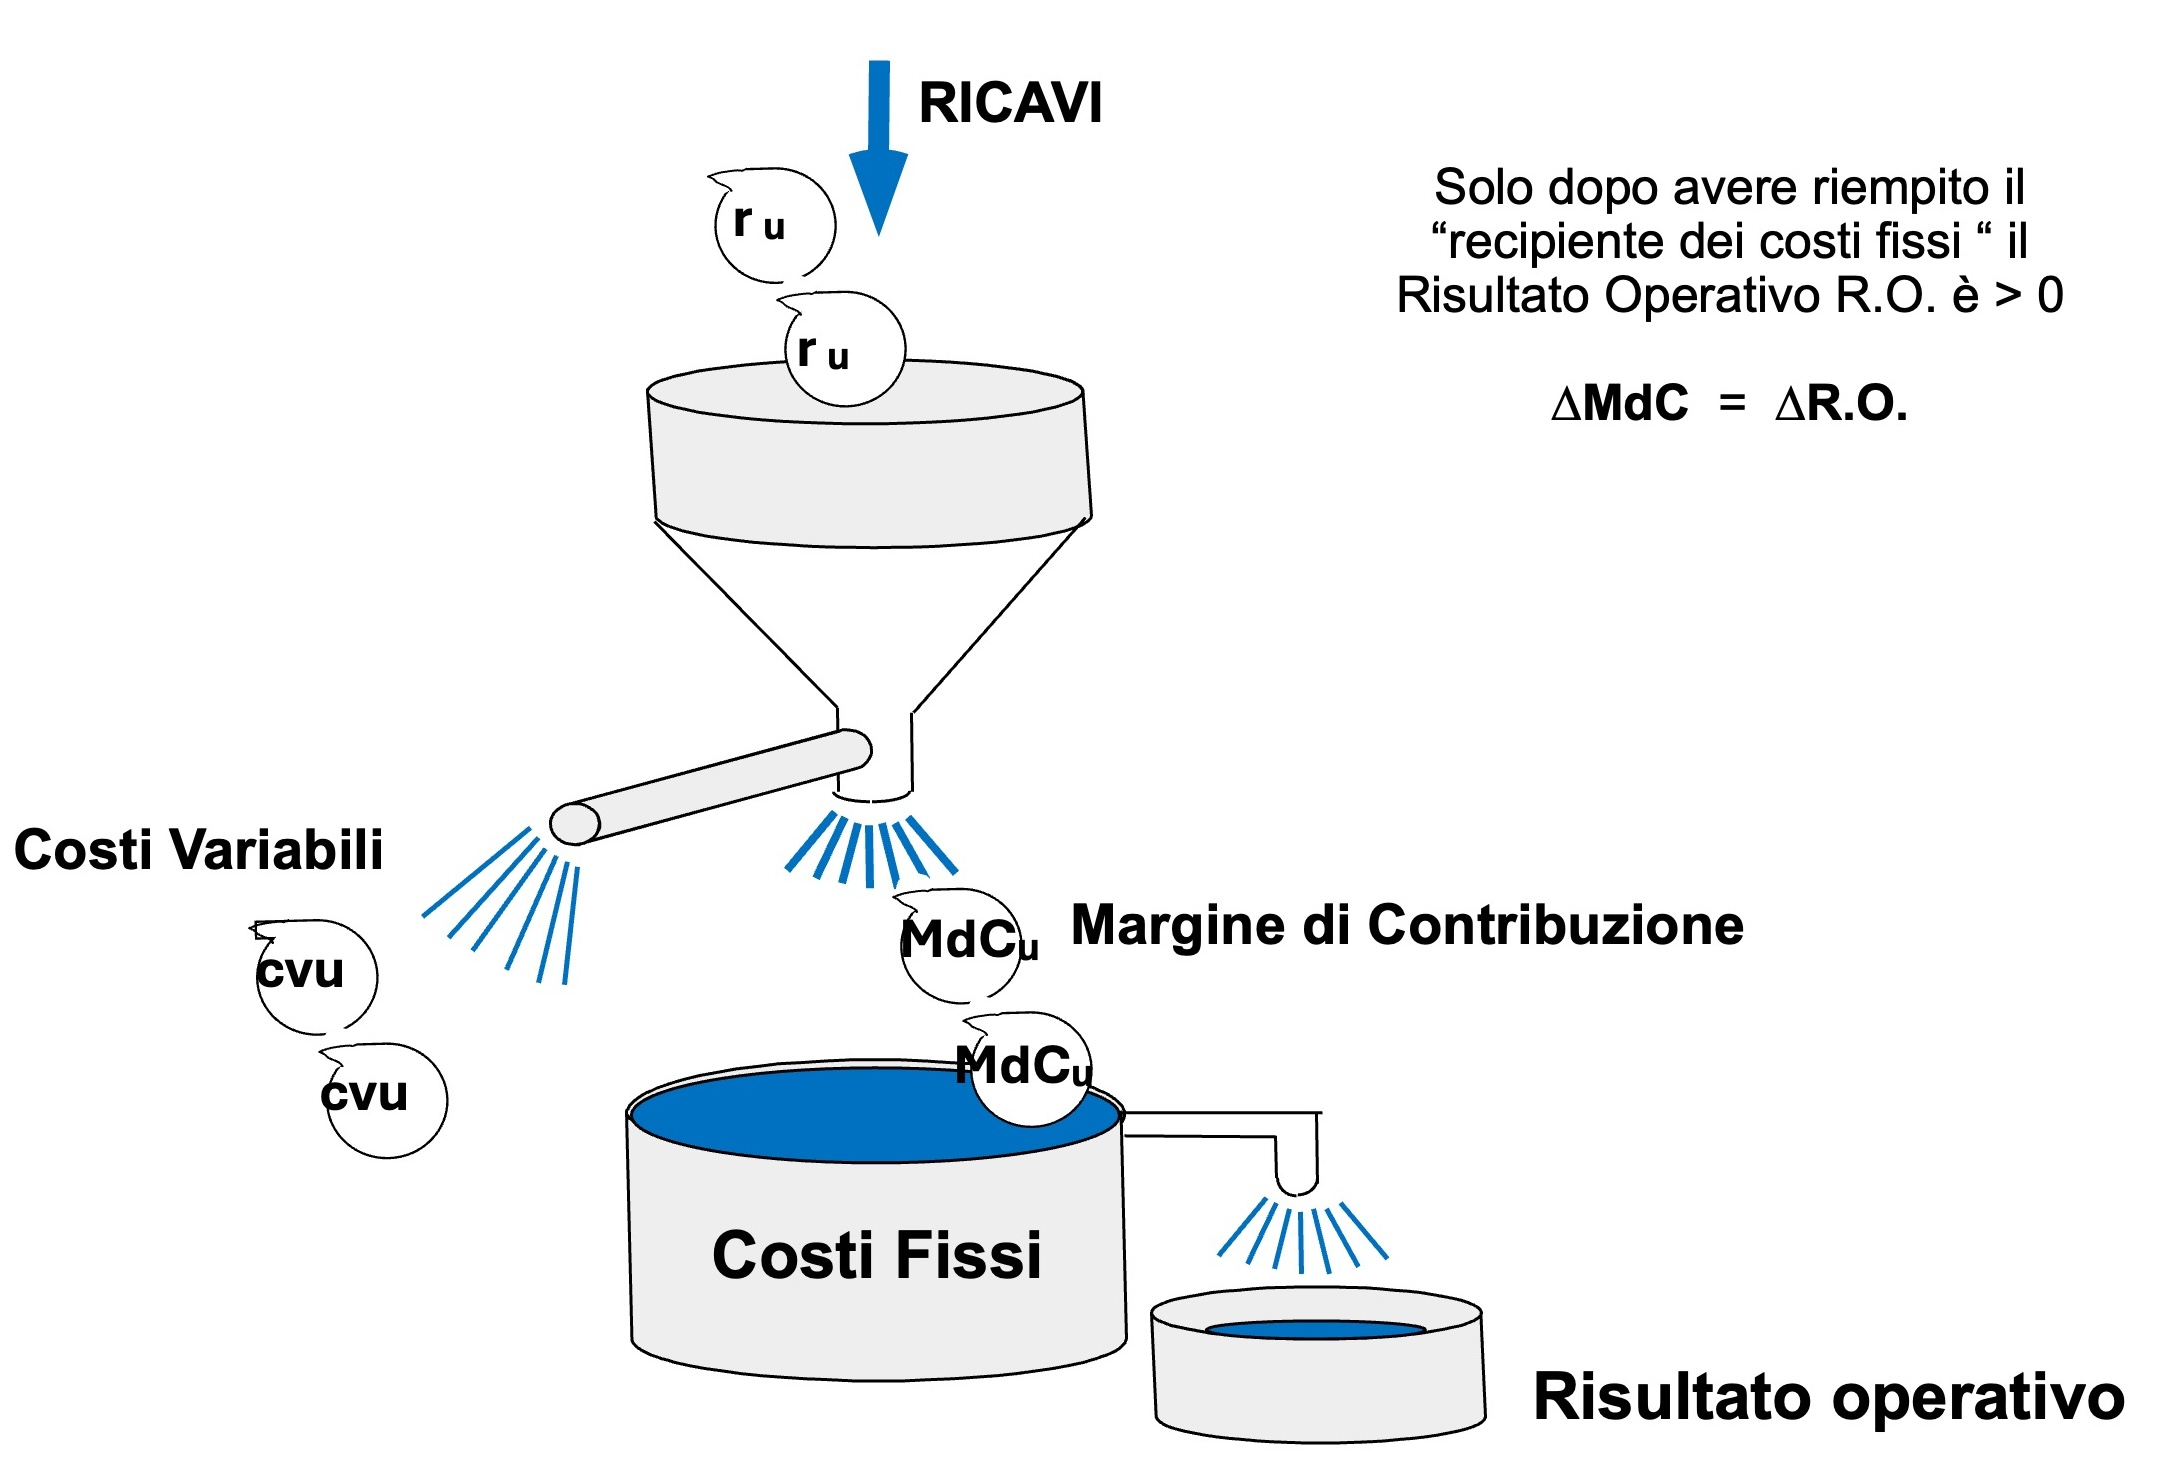
\includegraphics[width=0.7\textwidth]{src/Light/Margine di contribuzione.jpg}
    \caption{Margine di contribuzione e Reddito}
\end{figure}
\newpage
\section{Conto economico a margine di contribuzione}
\'E un rendiconto preparato per valutare rapidamente l'effetto sul reddito di cambiamenti delle quantit\'a vendute o dei ricavi.
\begin{figure}[H]
    \centering
    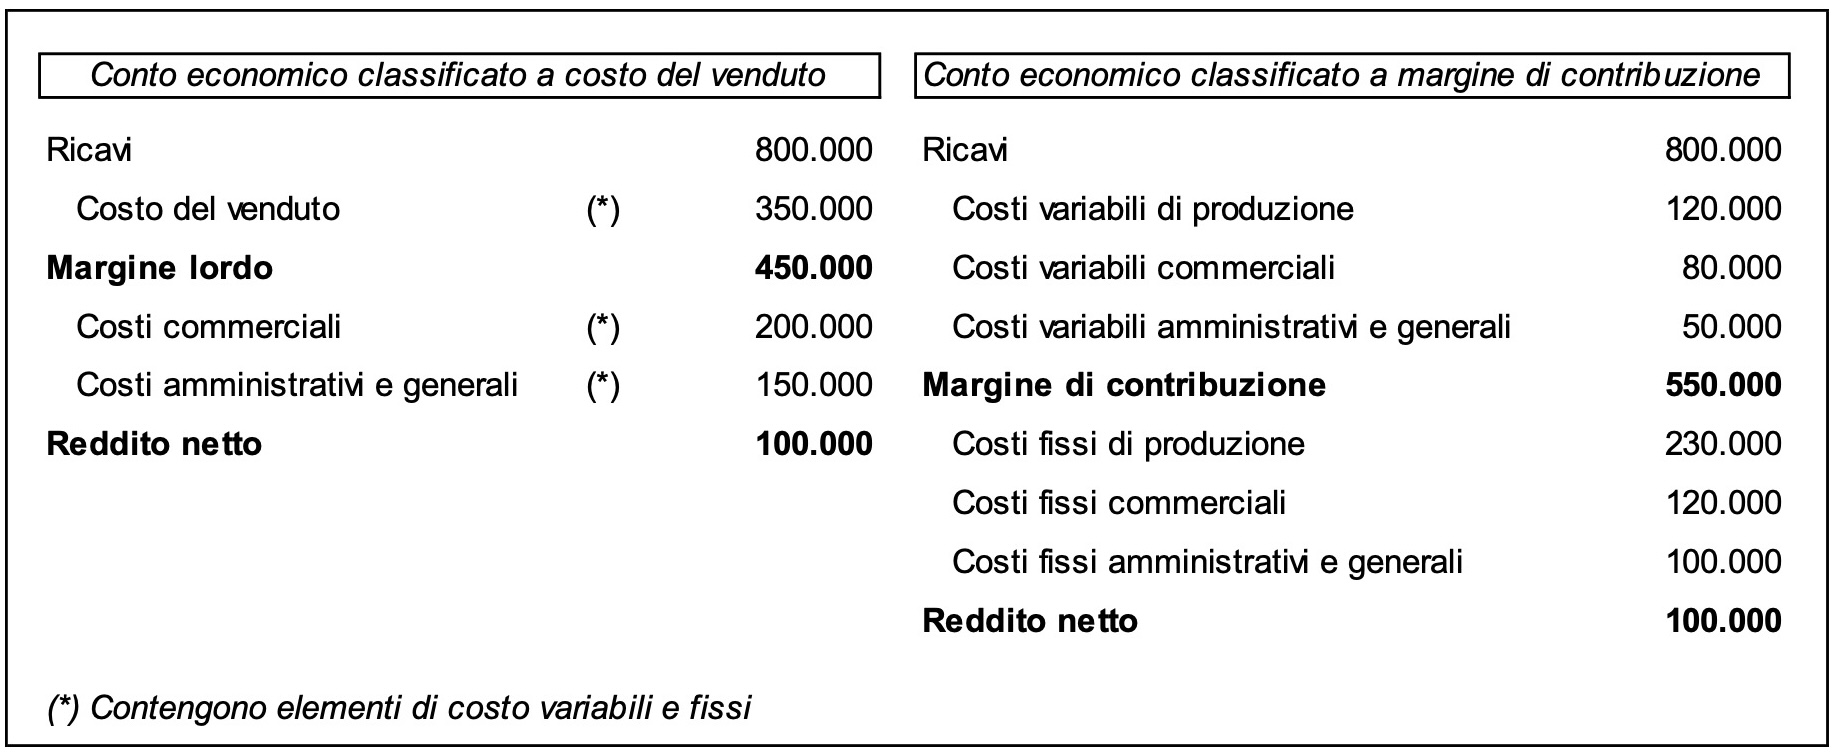
\includegraphics[width=0.8\textwidth]{src/Light/Conto economico a margine di contribuzione.jpg}
    \caption{Conto economico a margine di contribuzione}
\end{figure}
\begin{table}[H]
    \setlength{\extrarowheight}{12pt}
    \adjustbox{max width=\textwidth,center}{
        \centering
        \begin{tabular}{|l|l|l|}
            \hline
            \rowcolor{myblue}
            \textbf{Voce}                     & \textbf{Spiegazione}                   & \textbf{Voce}    \\
            \hline
            Ricavi                            & Ricavi totali                          & $RT$             \\
            Costi variabili                   & Costi variabili totali                 & $CVT$            \\
            \textbf{Margine di contribuzione} & Ricavi - Costi variabili               & $MdC = RT - CVT$ \\
            \hline
            Costi fissi totali                & Costi fissi totali                     & $CFT$            \\
            \textbf{Utile o Profitto}         & Margine di contribuzione - Costi fissi & $RT= MdC - CFT$  \\
            \hline
        \end{tabular}
    }
    \caption{Conto economico a margine di contribuzione}
\end{table}
\newpage
\section{Costi pieni}
\begin{itemize}
    \item \textbf{Costo} : \textbf{valorizzazione monetaria} delle risorse consumate per conseguire uno \textbf{scopo},(\textbf{Oggetto del costo}).
    \item \textbf{Costo pieno} : somma di :
          \begin{itemize}
              \item \textbf{Costo diretto} : costo che può essere \textbf{direttamente} ricondotto all’oggetto del costo.
              \item \textbf{Costo indiretto} : costo che \textbf{non} può essere \textbf{direttamente} ricondotto all’oggetto del costo.
          \end{itemize}
\end{itemize}
\subsection{Costruzione costo pieno di un prodotto}
\begin{figure}[H]
    \centering
    \begin{tikzpicture}[node distance=4cm, auto]
        % Styles
        \tikzstyle{box} = [rectangle, draw, text width=8em, text centered, minimum height=2.5em]
        \tikzstyle{line} = [draw, -latex']

        % Nodes
        \node [box] (costipieni) {Costi Pieni};
        \node [box, below left of=costipieni] (costopienoproduzione) {Costo Pieno di Produzione (\textit{Inventariabili})};
        \node [box, below right of=costipieni] (costiperiodo) {Costi di Periodo};

        \node [box, below right of=costopienoproduzione] (costitrasformazione) {Costi di Trasformazione};
        \node [box, below left of=costopienoproduzione] (materialidiretti) {Materiali Diretti};
        \node [box, below left of=costitrasformazione] (modiretta) {Costi Manodopera Diretta};
        \node [box, below of=costitrasformazione] (costiindiretti) {Costi Generali di Produzione};

        \node [box, below of=costiperiodo] (costicommerciali) {Costi Commerciali};
        \node [box, below right of=costiperiodo] (costiamministrativi) {Costi Amministrativi};
        % Lines
        \path[line] (costipieni) -- (costiperiodo);
        \path[line] (costipieni) -- (costopienoproduzione);
        \path[line] (costopienoproduzione) -- (costitrasformazione);
        \path[line] (costopienoproduzione) -- (materialidiretti);
        \path[line] (costitrasformazione) -- (modiretta);
        \path[line] (costitrasformazione) -- (costiindiretti);
        \path[line] (costiperiodo) -- (costicommerciali);
        \path[line] (costiperiodo) -- (costiamministrativi);

    \end{tikzpicture}
    \caption{Costruzione del costo pieno di un prodotto.}
\end{figure}
\begin{enumerate}
    \item \textbf{Costi pieni di produzione(inventariabili)}:
          \begin{enumerate}
              \item \textbf{Costi manodopera diretta} : costo del lavoro \textbf{direttamente} impiegato nella produzione di un prodotto.
              \item \textbf{Costi generali(indiretti) di produzione} (\textit{overhead cost}) : costi che \textbf{non} possono essere \textbf{direttamente} ricondotti alla produzione di un prodotto.
              \item \textbf{Costi materiali diretti} : costo dei materiali \textbf{direttamente} impiegati nella produzione di un prodotto.
          \end{enumerate}
    \item \textbf{Costi di periodo(operativi)} :
          \begin{enumerate}
              \item \textbf{Costi commerciali} : costi sostenuti per la vendita di un prodotto.
              \item \textbf{Costi amministrativi} : costi sostenuti per la gestione dell’azienda.
          \end{enumerate}
\end{enumerate}
\newpage
\section{Allocazione dei costi}
Il processo di assegnazione dei \textbf{costi indiretti} ai prodotti.
\subsection{How to}
I costi indiretti o generali sono allocati per mezzo di un \textbf{coefficiente di allocazione}, che può essere:
\begin{itemize}
    \item \textbf{Fisico} : il coefficiente di allocazione è una misura fisica.
    \item \textbf{Monetario} : il coefficiente di allocazione è una misura monetaria.
\end{itemize}
\begin{table}[H]
    \setlength{\extrarowheight}{12pt}
    \adjustbox{max width=\textwidth,center}{
        \centering
        \begin{tabular}{|l|c|l|l|}
            \hline
            \rowcolor{myblue}
            \textbf{Formula}            & \textbf{Equazione}                                                             & \textbf{Spiegazione}               & \textbf{Osservazioni}    \\
            \hline
            Coefficiente di allocazione & $ca = \displaystyle\frac{ \text{Costi Indiretti}}{\text{Base di allocazione}}$ & Costo indiretto per unità prodotta & $\textcolor{myblue}{ca}$ \\
            \hline
        \end{tabular}
    }
\end{table}
\subsection{Basi di allocazione}
Cosa si intende per base di allocazione? Una base di allocazione è una misura che riflette il consumo di risorse da parte di un prodotto.
\begin{itemize}
    \item \textbf{Fisiche} : \begin{itemize}
              \item \textbf{Unità prodotte} : numero di unità prodotte.
              \item \textbf{Ore di manodopera} : numero di ore di manodopera impiegate.
              \item \textbf{Ore macchina} : numero di ore macchina impiegate.
              \item \textbf{Metri quadri} : metri quadri occupati.
              \item \textbf{Peso} : peso del prodotto.
          \end{itemize}
    \item \textbf{Monetarie} :
          \begin{itemize}
              \item \textbf{Costo manodopera diretta}
              \item \textbf{Costo materiali diretti}
              \item \textbf{Costo manodopera diretta e materiali diretti}
          \end{itemize}
\end{itemize}

\newpage

\section{Costo standard}
\subsection*{Costo standard}
Sono costi prefissati e utilizzati per la valutazione delle prestazioni. Vengono confrontati con i costi effettivi per determinare le varianze.
\subsubsection*{Scheda dei costi standard}
\begin{figure}[H]
    \centering
    \begin{tikzpicture}[node distance=4cm]
        \tikzstyle{box} = [rectangle, draw,minimum width=3cm, minimum height=1cm, text centered]
        \node (scheda) [box] {Scheda dei costi standard};
        \node (distinta) [box, below left of=scheda] {Distinta base};
        \node (operazioni) [box, below right of=scheda] {Operazioni di trasformazione};
        \draw [->] (scheda) -- (distinta);
        \draw [->] (scheda) -- (operazioni);
    \end{tikzpicture}
\end{figure}
\textbf{Distinta base}: elenco dei materiali diretti e delle componenti necessarie per la produzione di un prodotto.
\textbf{Operazioni di trasformazione}: elenco delle operazioni necessarie per trasformare i materiali diretti in prodotto finito.
\begin{table}[H]
    \centering
    \begin{tabular}{|l|l|l|l|}
        \hline
        \rowcolor{myblue}
        \multicolumn{4}{|c|}{\textbf{Scheda dei costi standard}}                                                                    \\
        \rowcolor{myblue}
        \multicolumn{4}{|l|}{\textbf{Distinta base}}                                                                                \\
        \hline
        \rowcolor{myblue}
        \textbf{Articolo}                  & \textbf{Quantità standard} & \textbf{Prezzo unitario standard} & \textbf{Costo totale} \\
        \hline
        Materiale X                        & 120 cm                     & 0,05 \euro                        & 6,00 \euro            \\
        Componente Y                       & 2 unità                    & 1,00 \euro                        & 2,00 \euro            \\
        \textbf{Totale materiali diretti}  &                            &                                   & 8,00 \euro            \\
        \hline
        \rowcolor{myblue}
        \multicolumn{4}{|l|}{\textbf{Operazizoni di trasformazione}}                                                                \\
        \rowcolor{myblue}
        \textbf{Operazione}                & \textbf{Quantità standard} & \textbf{Costo unitario standard}  & \textbf{Costo totale} \\
        \hline
        Taglio                             & 1 ora                      & 10,00 \euro                       & 10,00 \euro           \\
        Assemblaggio                       & 1 ora                      & 10,00 \euro                       & 10,00 \euro           \\
        \textbf{Totale manodopera diretta} &                            &                                   & 20,00 \euro           \\
        \hline
        \textbf{Costo standard}            &                            &                                   & 28,00 \euro           \\
        \hline
    \end{tabular}
    \caption{Esempio di operazioni di trasformazione}
\end{table}
\subsubsection*{Costi effettivi}
Sono i costi effettivamente sostenuti per la produzione di un prodotto.
\subsection{Analisi delle varianze}
\subsubsection*{Scostamento o Varianza}
\'E la differenza tra due numeri
\begin{align*}
     & \text{Varianza} = \text{Costi standard} - \text{Costi effettivi} \\
\end{align*}
\subsubsection*{Varianza materiali diretti}
\paragraph{Esempio}
Un impresa ha acquistato $\num{26000}\ \unit{kg}$ a $\num{2}\ \frac{\text{\euro}}{\unit{kg}}$

\newpage

\section{Investimenti}
\paragraph{Analisi degli investimenti} : L' \textit{analisi degli investimenti} o \textit{budget di capitale} è un elenco degli investimenti che un'organizzazione intende realizzare.
\paragraph{Investire} : impiegare risorse finanziarie per acquistare beni o servizi che si prevede generino benefici futuri.
\paragraph{Punti chiave} :
\begin{itemize}
    \item Impiego di capitale
    \item Durata lunga
    \item Bassa reversibilità
    \item Rischio
\end{itemize}
\paragraph{Investimenti tipici con incertezza crescente} :
\begin{itemize}
    \item Sostituzione di macchinari o impianti
    \item Automazione
    \item Espansione
    \item Ampliamento dell'offerta
\end{itemize}

\paragraph{Valore del denaro nel tempo} : "Un euro oggi vale più di un euro domani", se non investo domani ho un euro, se investo domani ho un euro più gli interessi, potrei generare un \textbf{flusso di cassa}.

\paragraph{Flusso di cassa} : è un insieme di entrate e uscite di denaro in un periodo di tempo, nell'analisi degli investimenti non si ragiona in termini di reddito (costo - ricavo) ma in termini di flusso di cassa (entrata - uscita).

\paragraph{Rendiconto dei flussi di cassa} : Partendo dal bilancio di esercizio, in genere il \textbf{conto economico (a costo del venduto)}, si aggiungono le voci che non hanno effetto sul flusso di cassa e si eliminano le voci che non hanno effetto sul flusso di cassa.

\paragraph{Costo opportunità del capitale}
Per rendere comparabili flussi di cassa che hanno manifestazione in momenti differenti è necessario introdurre il \textbf{costo di opportunità del capitale}, $ r $, ossia il rendimento che si otterrebbe investendo in un progetto alternativo di mercato avente lo stesso livello di rischio.
\begin{align*}
    \text{Costo opportunità del capitale} = \textcolor{myblue}{r}
\end{align*}

\paragraph{Confronto tra flussi di cassa} : Per confrontare flussi di cassa che hanno manifestazione in momenti differenti è necessario portarli a un unico momento temporale, si può fare in due modi: \textbf{attualizzazione} e \textbf{capitalizzazione}.
\begin{itemize}
    \item $\displaystyle \frac{1}{(1+\textcolor{myblue}{r})} = $ Coefficiente di \textbf{Attualizzazione} : è il fattore di attualizzazione che permette di portare un flusso di cassa futuro al tempo zero.
    \item $\displaystyle (1+\textcolor{myblue}{r}) = $ Coefficiente di \textbf{Capitalizzazione} : è il fattore di capitalizzazione che permette di portare un flusso di cassa al tempo zero a un tempo futuro.
\end{itemize}
\begin{table}[H]
    \centering
    \setlength{\extrarowheight}{6pt}
    \begin{tabular}{|l|l|c|}
        \rowcolor{myblue}
        \hline
        \textbf{Voce}                           & \textbf{Spiegazione}                                    & \textbf{Formula}                                                   \\
        \hline
        \textbf{Costo opportunità del capitale} &                                                         & $\textcolor{myblue}{r}$                                            \\
        \textbf{Valore attuale}                 & Valore futuro $\cdot$ Coefficiente di Attualizzazione   & VA =  $\displaystyle \frac{\text{F}}{(1+\textcolor{myblue}{r})^n}$ \\
        \textbf{Valore futuro o Montante}       & Valore attuale $\cdot$ Coefficiente di Capitalizzazione & F = VA $\cdot (1+\textcolor{myblue}{r})^n$                         \\
        \hline
    \end{tabular}
    \caption{Confronto tra flussi di cassa}
\end{table}

\begin{figure}[H]
    \centering
    \begin{tikzpicture}[scale = 1]
        \tikzstyle{box} = [rectangle, draw,minimum width=3cm, minimum height=1cm, text centered]
        % Draw t-axis
        \draw[-latex] (-4,0) -- (10,0) node[below] {$t$};
        % Draw vertical lines
        \draw[-latex] (0,-0.5) -- (0,4) node[left] {$F$};
        % Draw lines for time points
        \draw(2,0) -- (2,-1) node[left]{};
        \draw(4,0) -- (4,-1.2) node[left]{};
        \draw(8,0) -- (8,-1.4) node[left]{};
        % Draw arrows for cash flows
        \draw[-latex](2,-1) -- (0,-1) node[left]{};
        \draw[-latex](4,-1.2) -- (0,-1.2) node[left]{};
        \draw[-latex](8,-1.4) -- (0,-1.4) node[left]{};
        % Label time points
        \node[below right] at (0,0) {$0$};
        \node[below right] at (2,0) {$t_1$};
        \node[below right] at (4,0) {$t_2$};
        \node[below right] at (6,0) {$...$};
        \node[below right] at (8,0) {$t_n$};
        % Optionally, label the height of the bars if known
        \node[above] at (0,0.1) {$F_0=VA_0$};
        \node[above] at (2,0.5) {$F_1$};
        \node[above] at (4,1) {$F_2$};
        \node[above] at (8,3) {$F_n$};
        % Add rectangles for future cash flows
        \fill[red] (0-0.2,0) rectangle ++(0.4,0.1);   % Width of 0.4, height based on F1
        \fill[red] (2-0.2,0) rectangle ++(0.4,0.5);   % Width of 0.4, height based on F1
        \fill[red] (4-0.2,0) rectangle ++(0.4,1);     % Width of 0.4, height based on F2
        \fill[red] (8-0.2,0) rectangle ++(0.4,3);     % Width of 0.4, height based on Fn
        % NPV formula box
        \node (VA) [box] at (-2,-1) {$\text{VA}_t = \displaystyle \frac{F_t}{(1+r)^t} $};
    \end{tikzpicture}
    \caption{Operazione di attualizzazione di flussi di cassa futuri}
    \begin{tikzpicture}[scale = 1,
            declare function={
                    f(\x) = 30/((1+0.02)^(\x));
                    g(\x) = 30*((1+0.02)^(\x));
                }]
        \def\p{1.428}
        \begin{axis}
            [
                xlabel={\( \ tempo \)},
                ylabel={\( flussi\ di\ cassa \)},
                xmin=-30, xmax=190,
                ymin=-30, ymax=90,
                grid=both,
                axis lines=middle,
                axis line style=->,
                grid style={line width=.1pt, draw=gray!10},
                major grid style={line width=.2pt,draw=gray!50},
                minor tick num=3,
                enlargelimits={abs=0.5},
                xlabel style={at={(ticklabel* cs:1)}, anchor=north west},
                ylabel style={at={(ticklabel* cs:1)}, anchor=south west},
                samples=100,
                unbounded coords=jump,
                legend pos=south east,
            ]
            \addplot [domain=0:80, ultra thick, smooth, color=red]{g(x)};
            \addplot [domain=0: 190, ultra thick, smooth, color=myblue]{f(x)};
            \legend{$F$, $VA$}
        \end{axis}
    \end{tikzpicture}
    \caption{Visualizzazione del flusso di cassa attualizzato e del flusso di cassa futuro}
\end{figure}

\subsection*{Valore Attuale Netto (VAN)}
La differenza tra il valore attuale dei flussi di cassa generati dall’investimento e l’impegno iniziale di risorse monetarie si chiama valore attuale netto o VAN.
Consiste nell'attualizzazione dei flussi di cassa generati da un investimento.
\paragraph{Formulazione del VAN}
\begin{align*}
     & \text{VAN} = -I + \sum_{t=0}^{n} \frac{F_t}{(1 + r)^t}                                                \\
     & \text{VAN} = -I + \displaystyle \frac{F_1}{(1+r)^1} + \frac{F_2}{(1+r)^2} + ... + \frac{F_n}{(1+r)^n}
\end{align*}
Dove:
\begin{itemize}
    \item \(F_t\) rappresenta i flussi di cassa futuri al tempo \(t_{-esimo}\), ovvero il Montante al tempo \(t_{-esimo}\).
    \item \(r\) è il costo opportunità del capitale
    \item \(I\) è l'investimento iniziale
\end{itemize}
\paragraph{Decisione di investimento} :
\begin{itemize}
    \item Se VAN $>$ 0, l'investimento è conveniente.
    \item Se VAN $<$ 0, l'investimento non è conveniente.
    \item Se VAN $=$ 0, l'investimento è indifferente.
\end{itemize}
\begin{figure}[H]
    \centering
    \begin{tikzpicture}[scale = 1,
            declare function={
                    f(\x) = 3/((1+0.7)^(\x)) -2;
                    g(\x) = -2;
                }]
        \def\p{0.76}
        \begin{axis}
            [
                xlabel={\( \ r \)},
                ylabel={\( VAN \)},
                xmin=-4, xmax=6,
                ymin=-4, ymax=4,
                grid=both,
                axis lines=middle,
                axis line style=->,
                grid style={line width=.1pt, draw=gray!10},
                major grid style={line width=.2pt,draw=gray!50},
                minor tick num=3,
                enlargelimits={abs=0.5},
                xlabel style={at={(ticklabel* cs:1)}, anchor=north west},
                ylabel style={at={(ticklabel* cs:1)}, anchor=south west},
                samples=100,
                unbounded coords=jump,
                legend pos=south east,
            ]
            \addplot [domain=0: 6, ultra thick, smooth, color=myblue]{f(x)};
            \addplot [domain=-4: 0, ultra thick, dashed, color=myblue]{f(x)};
            \addplot [domain=-4: 6, thick , dashed]{g(x)};
            \node [below right] at (axis cs: 0, -2) {-I};
            \filldraw (axis cs:0,-2) circle (1.5pt);
            \legend{$VAN$}
        \end{axis}
    \end{tikzpicture}
    \caption{Visualizzazione del VAN}
\end{figure}
Nota che per avere il VAN maggiore di zero i fattori che influenzano il VAN sono:
\begin{itemize}
    \item Aumentare i flussi di cassa futuri
    \item Diminuire il costo opportunità del capitale
    \item Diminuire l'investimento iniziale
    \item Aumentare il tempo di durata dell'investimento
\end{itemize}
\paragraph{Rendita perpetua} : La rendita perpetua, o \textit{perpetuity}, è una serie di flussi di cassa di uguale importo che si ripetono all'infinito. È un concetto utilizzato in finanza per valutare il valore presente di flussi di cassa che si prevede continueranno in eterno. Tipicamente, si considera in contesti come valutazioni immobiliari (affitti) o titoli finanziari che pagano dividendi costanti.
\begin{align*}
    \text{Valore Attuale (VA) della rendita perpetua} = \frac{F}{r}
\end{align*}
Dove:
\begin{itemize}
    \item \(F\) rappresenta l'importo fisso del flusso di cassa o pagamento che si riceve periodicamente (per esempio, un affitto annuale da un immobile).
    \item \(r\) è il tasso di sconto o il costo opportunità del capitale, che riflette il ritorno che si potrebbe ottenere da investimenti alternativi di rischio simile.
\end{itemize}
\paragraph{Esempio di rendita perpetua con affitto} : Supponiamo di possedere un appartamento che affittiamo per 10.000\euro all'anno. Se consideriamo un tasso di sconto annuo del 5\%, il valore attuale di questi flussi di cassa perpetui è calcolato come:
\[ VA = \frac{10000}{0.05} = 200000 \]
Quindi, ricevere 10.000\euro all'anno per sempre, scontati al 5\%, è equivalente a ricevere 200.000\euro oggi. Questo valore attuale ci offre una prospettiva sul valore attuale di flussi di cassa futuri infiniti, permettendoci di confrontare questa opzione di investimento con altre disponibili.

\newpage

\section*{Metodi Alternativi al VAN}
\paragraph{TIR (Tasso Interno di Rendimento)}
Il \textbf{TIR} è quel valore del tasso di attualizzazione  che rende il \textbf{VAN dell'investimento pari a zero}. È un indicatore della redditività di un progetto.
Negli investimenti scelgo il progetto con il TIR maggiore.
\begin{align*}
     & \text{TIR} = \textcolor{myblue}{r} \text{ tale che } \text{VAN} = 0                                       \\
     & \text{TIR} = \text{VAN} = \sum_{t=0}^{n} \frac{F_t}{(1 + \textcolor{myblue}{r})^t} - I = 0                \\
     & \text{TIR} = -I + \displaystyle \frac{F_1}{(1+r)^1} + \frac{F_2}{(1+r)^2} + ... + \frac{F_n}{(1+r)^n} = 0
\end{align*}
\begin{figure}[H]
    \centering
    \begin{tikzpicture}[scale = 1,
            declare function={
                    f(\x) = 3/((1+0.7)^(\x)) -2;
                    g(\x) = -2;
                }]
        \def\p{0.76}
        \begin{axis}
            [
                xlabel={\( \ r \)},
                ylabel={\( VAN \)},
                xmin=-4, xmax=6,
                ymin=-4, ymax=4,
                grid=both,
                axis lines=middle,
                axis line style=->,
                grid style={line width=.1pt, draw=gray!10},
                major grid style={line width=.2pt,draw=gray!50},
                minor tick num=3,
                enlargelimits={abs=0.5},
                xlabel style={at={(ticklabel* cs:1)}, anchor=north west},
                ylabel style={at={(ticklabel* cs:1)}, anchor=south west},
                samples=100,
                unbounded coords=jump,
                legend pos=south east,
            ]
            \addplot [domain=0: 6, ultra thick, smooth, color=myblue]{f(x)};
            \addplot [domain=-4: 0, ultra thick, dashed, color=myblue]{f(x)};
            \addplot [domain=-4: 6, thick , dashed]{g(x)};
            \node [above right, color=red] at (axis cs: \p, 0) {\(TIR\)};
            \node [below right] at (axis cs: 0, -2) {-I};
            \filldraw[color=red] (axis cs:\p,{f(\p)}) circle (1.5pt);
            \filldraw (axis cs:0,-2) circle (1.5pt);
            \legend{$VAN$}
        \end{axis}
    \end{tikzpicture}
    \caption{Visualizzazione del TIR}
\end{figure}
\paragraph{Decisione di investimento} :
\begin{itemize}
    \item Se TIR $>$ r, $\Rightarrow$ VAN $>0$ l'investimento è conveniente .
    \item Se TIR $<$ r, $\Rightarrow$ VAN $<0$ l'investimento non è conveniente.
    \item Se TIR $=$ r, $\Rightarrow$ VAN $=0$ l'investimento è indifferente.
\end{itemize}
Ricordiamo che r è il costo opportunità del capitale, ovvero il rendimento che si otterrebbe investendo in un progetto alternativo di mercato avente lo stesso livello di rischio.
\paragraph{I limiti del TIR}
\begin{itemize}
    \item Il TIR non ha un significato economico semplice e, soprattutto, non rappresenta il rendimento ottenuto sull’investimento cioè sull’esborso iniziale
          (il TIR rappresenterebbe il rendimento dell’investimento solo se si riuscissero a reinvestire gli incassi a un rendimento pari al TIR)
    \item Non è quindi possibile, nel caso più generale, stabilire tra due proposte di investimento quale sia la più conveniente confrontando i corrispondenti valori dei TIR
    \item Il TIR non è univocamente determinato
\end{itemize}
\newpage
\subsection*{Tempo di Recupero (Payback Period)}
Il \textbf{Tempo di Recupero} è il periodo necessario affinché il valore cumulato dei flussi di cassa generati da un investimento eguagli o superi l'importo dell'investimento iniziale. Questa metrica è utilizzata per valutare la rapidità con cui un investimento può ripagarsi. La formula per il calcolo del Tempo di Recupero è:
\[
    \text{Tempo di Recupero} = \text{Anno in cui il flusso di cassa cumulato diventa non negativo}
\]
Per calcolarlo precisamente, si sommano i flussi di cassa annuali fino a quando il totale non raggiunge l'importo investito inizialmente. La formula dettagliata, considerando flussi di cassa annuali costanti, è:

\[
    \text{Tempo di Recupero} = \frac{\text{Investimento Iniziale}}{\text{Flusso di Cassa Annuale}}
\]
Nel caso di flussi di cassa non costanti, il calcolo diventa più complesso e richiede di sommare i flussi di cassa anno per anno fino a quando l'investimento iniziale non è completamente recuperato.
Nonostante sia ampiamente utilizzato per la sua semplicità, il Tempo di Recupero presenta delle limitazioni:
\begin{itemize}
    \item Non tiene conto del valore temporale del denaro. Flussi di cassa futuri non sono scontati e quindi valgono tanto quanto i flussi di cassa presenti.
    \item Ignora i flussi di cassa che si verificano dopo il punto di recupero. Ciò significa che non fornisce informazioni sulla redditività totale o sul valore di un investimento oltre il periodo di payback.
\end{itemize}
Questo metodo è particolarmente utile per valutare la liquidità e il rischio di un investimento, ma dovrebbe essere utilizzato insieme ad altre metriche finanziarie per una valutazione completa della convenienza di un investimento.
\subsection*{Rendimento Medio Contabile}
\'E una misura della redditività di un investimento basata sui valori contabili. Esso indica quanto reddito è stato generato da ogni unità di valore contabile medio investito. La formula per calcolare il RMC è:

\[
    RMC = \frac{\text{Utile Netto Medio}}{\text{Valore Contabile Medio Netto dell'Investimento}}
\]

dove:
\begin{itemize}
    \item \textbf{Utile Netto Medio} è calcolato come:
          \[
              \text{Utile Netto Medio} = \frac{\sum_{i=1}^{n} \text{Utile Netto Annuale}_i}{n}
          \]
          dove $n$ rappresenta il numero di anni considerati per il calcolo.

    \item \textbf{Valore Contabile Medio Netto dell'Investimento} è calcolato come:
          \[
              \text{Valore Contabile Medio Netto dell'Investimento} = \frac{\text{Valore Contabile Iniziale} + \text{Valore Contabile Finale}}{2}
          \]
          Questo valore rappresenta la media del valore contabile all'inizio e alla fine del periodo considerato.
\end{itemize}
\newpage
\section{Domande di esame}
\begin{enumerate}
    \item Quale dei seguenti indici fornisce informazioni circa la capacità dell'impresa di fare fronte in modo adeguato a passività in scadenza nel breve periodo?
          \begin{itemize}
              \item[\checkmark] A. Indice di liquidità
              \item[\sout{B.}] ROA
              \item[\sout{C.}] ROE
              \item[\sout{D.}] Indice di indebitamento
          \end{itemize}

    \item Contabilmente, dobbiamo registrare una minusvalenza quando:
          \begin{itemize}
              \item[\sout{A.}] Cedendo una immobilizzazione, il costo storico non è stato completamente ammortizzato
              \item[\sout{B.}] Cedendo un bene immobilizzato, la perdita di valore legata al valore di mercato non è stata precedentemente ammortizzata
              \item[\checkmark] C. Cedendo un bene immobilizzato, il prezzo di vendita risulta inferiore al relativo costo storico al netto del fondo ammortamento
              \item[\sout{D.}] Cedendo un bene immobilizzato, il prezzo di vendita risulta superiore al relativo costo storico al netto del fondo ammortamento
          \end{itemize}

    \item Nella valutazione di investimenti, VAN e TIR danno lo stesso risultato quando:
          \begin{itemize}
              \item[\sout{A.}] i progetti si escludono a vicenda
              \item[\checkmark] B. viene valutato un solo progetto
              \item[\sout{C.}] il capitale da investire è razionato (ovvero limitato)
              \item[\sout{D.}] il tasso di attualizzazione rifletto solo il rischio sistematico
          \end{itemize}

    \item Quale tra lo seguenti informazioni il bilancio di esercizio non è in grado di fornire all'osservatore?
          \begin{itemize}
              \item[\sout{A.}] La situazione debitoria
              \item[\sout{B.}] Il capitale di rischio
              \item[\checkmark] C. Il valore di mercato dell'impresa
              \item[\sout{D.}] L'efficienza operativa
          \end{itemize}

    \item Concettualmente, cosa rappresenta l'avviamento?
          \begin{itemize}
              \item[\sout{A.}] È una voce di conto economica da inserire tra, costi di periodo
              \item[\checkmark] B. La differenza tra il prezzo d'acquisto pagato per un'azienda ed il suo valore contabile
              \item[\sout{C.}] Una voce positiva da inserire in conto economico nella gestione accessoria
              \item[\sout{D.}] Una voce delle immobilizzazioni materiali in stato patrimoniale
          \end{itemize}

    \item Nell'analisi del punto di pareggio, un aumento del margine di contribuzione unitario comporta:
          \begin{itemize}
              \item[\sout{A.}] Un aumento proporzionale del costo variabile unitario
              \item[\sout{B.}] Un aumento dei costi fissi, a parità di quantità vendute
              \item[\sout{C.}] Non ha nessun effetto sull'utile dell'impresa, a parità di quantità vendute
              \item[\checkmark] D. Una diminuzione della quantità di pareggio, a parità di costi fissi
          \end{itemize}
\end{enumerate}
\newpage
\begin{enumerate}
    \item Quale delle seguenti affermazioni è falsa in riferimento al TIR come criterio di valutazione degli investimenti?
          \begin{itemize}
              \item[\sout{A.}] È un tasso che potrebbe non essere l'unico per un progetto.
              \item[\sout{B.}] Nel valutare due progetti di investimento alternativi, il confronto dei TIR dei due progetti potrebbe dare indicazioni fuorvianti.
              \item[\checkmark] È il tasso che misura il rendimento dell'investimento.
              \item[\sout{C.}] È il tasso di sconto che rende nulla il valore del VAN.
          \end{itemize}

    \item Nella valutazione di un investimento con la formula del VAN, il costo opportunità del capitale può essere assimilato a:
          \begin{itemize}
              \item[\sout{A.}] Il rendimento garantito dai titoli di stato.
              \item[\sout{B.}] Il rendimento garantito da un investimento alternativo sicuro.
              \item[\sout{C.}] Il rendimento garantito da un portafoglio di titoli azionari dello stesso settore dell'impresa in questione.
              \item[\checkmark] Il rendimento garantito da un investimento alternativo caratterizzato da livello di rischio comparabile.
          \end{itemize}
    \item Quale è il valore attuale di una rendita perpetua basata su una rata annuale costante di 10.000 euro, considerando un costo opportunità del capitale del 10\%?
          \begin{itemize}
              \item[\sout{A.}] 1.000 euro.
              \item[\checkmark] 100.000 euro.
              \item[\sout{B.}] 1.000.000 euro.
              \item[\sout{C.}] 200.000 euro.
          \end{itemize}

    \item In una scelta tra investimenti alternativi, l'investimento più conveniente da un punto di vista economico-finanziario da scegliere dovrebbe essere sempre:
          \begin{itemize}
              \item[\sout{A.}] L'investimento con il livello di rischio più basso.
              \item[\sout{B.}] L'investimento che garantisce un payback più breve.
              \item[\sout{C.}] L'investimento con il valore di TIR più alto.
              \item[\checkmark] L'investimento con il valore del VAN più alto.
          \end{itemize}

    \item Tra i criteri di valutazione degli investimenti alternativi al VAN, il rendimento medio contabile di un progetto di investimento è:
          \begin{itemize}
              \item[\sout{A.}] Il rapporto tra flussi di cassa medi del progetto e il valore dell'esborso iniziale dell'investimento.
              \item[\sout{B.}] Il rapporto tra il reddito medio contabile del progetto e il valore dell'esborso iniziale dell'investimento.
              \item[\checkmark] Il rapporto tra il reddito medio contabile del progetto e il valore medio contabile netto dell'investimento.
              \item[\sout{C.}] Il rapporto tra reddito medio contabile del progetto e ricavi totali medi del progetto.
          \end{itemize}
\end{enumerate}
\newpage
\begin{enumerate}
    \item La varianza di impiego dei materiali diretti:
          \begin{itemize}
              \item[\checkmark] È la differenza fra la quantità totale standard ed effettiva utilizzata, valorizzata al prezzo standard.
              \item[\sout{B.}] È sfavorevole se la prestazione economica è inadeguata.
              \item[\sout{C.}] Dipende dalla quantità di output programmata.
              \item[\sout{D.}] È la differenza fra prezzo unitario effettivo e standard dei materiali diretti, moltiplicata per la quantità effettiva utilizzata.
          \end{itemize}
    \item Per aumentare il margine di contribuzione totale un'impresa dovrebbe:
          \begin{itemize}
              \item[\sout{A.}] Ridimensionare la capacità produttiva in modo da recuperare efficienza.
              \item[\sout{B.}] Ridurre i costi fissi totali.
              \item[\sout{C.}] Ridurre il prezzo di vendita del prodotto.
              \item[\checkmark] Diminuire i costi variabili unitari.
          \end{itemize}
    \item Il costo pieno di produzione è composto dai seguenti costi:
          \begin{itemize}
              \item[\sout{A.}] Materiali diretti + manodopera diretta + provvigioni + costi di periodo allocati.
              \item[\sout{B.}] Materiali diretti + manodopera diretta + costi di periodo allocati.
              \item[\checkmark] Materiali diretti + manodopera diretta + costi indiretti industriali allocati.
              \item[\sout{C.}] Materiali diretti + manodopera diretta + provvigioni + costi di periodo allocati.
          \end{itemize}
    \item Ipotizzando l'uguaglianza tra volumi di produzione e volumi di vendita, il punto di pareggio (break-even point):
          \begin{itemize}
              \item[\checkmark] Rappresenta quel livello di attività che consente la copertura di tutti i costi variabili e di tutti i costi fissi, portando al pareggio economico.
              \item[\sout{A.}] Rappresenta il volume di produzione per il quale i ricavi totali uguagliano i costi fissi totali.
              \item[\sout{B.}] Cala al crescere dei costi fissi.
              \item[\sout{C.}] Rappresenta il volume di produzione per il quale l'azienda consegue un utile positivo.
          \end{itemize}
    \item La distinta base riporta:
          \begin{itemize}
              \item[\sout{A.}] I costi di trasformazione.
              \item[\sout{B.}] I costi dei materiali diretti e di trasformazione.
              \item[\sout{C.}] Lo scostamento dei costi dei materiali diretti.
              \item[\checkmark] Il costo a budget dei materiali diretti.
          \end{itemize}
\end{enumerate}

\end{document}